% !TeX spellcheck = en_US
\section{Experiments}

\subsection{Test setup}

Our method requires the phone to be able to use the BLE peripheral role, and the server needs to be able to use the central role.

The specific devices used are an iPhone 5 or a Nexus 5, as mobile device and a Raspberry Pi with a Logilink USB Bluetooth 4.0 dongle running Raspbian Linux\cite{ref:raspbian} as base station. See \cref{fig_solution_overview} for an overview.

The base station test system\cite{ref:Github} is build as a prototype using node.js\cite{ref:node} and the Noble node module.
On the iPhone 5 we used the app LightBlue\cite{ref:Lightblue} to advertise a BLE peripheral service.

%For more information see appendix \ref{appendix:codeused}

\subsection{Scenarios}

%The base scenario consists of a Raspberry Pi with custom software as the system.
The following experiment was conducted with the base station being static throughout the experiments.

A "noisy environment" is an environment with several wifi hotspots and many people moving around with phones having access to Bluetooth, data, etc.

A "regular environment" is a standard home environment.

During the experiments there was always a clear line of sight from the mobile phone to the base station. There was no interference by physical objects or humans between the mobile phone and the base station.

%The device in the test scenario is an iPhone 5 cell phone and other wearables and will be both static and moving depending on the test scenario.

\subsubsection{Dynamic distance}
\label{section:MovingTowardsSystem}
In order for nearby authentication to work a threshold, that determines if the user is close enough for authentication, must be set.

The purpose of this scenario is to observe the relation between distance and RSSI value to make it possible to  define  this threshold. This is done by measuring the RSSI value of a single device at different distances, allowing us to define how close the user needs to be in order to be authenticated as illustrated on \cref{fig_distance}.

\begin{figure}
	\centering
	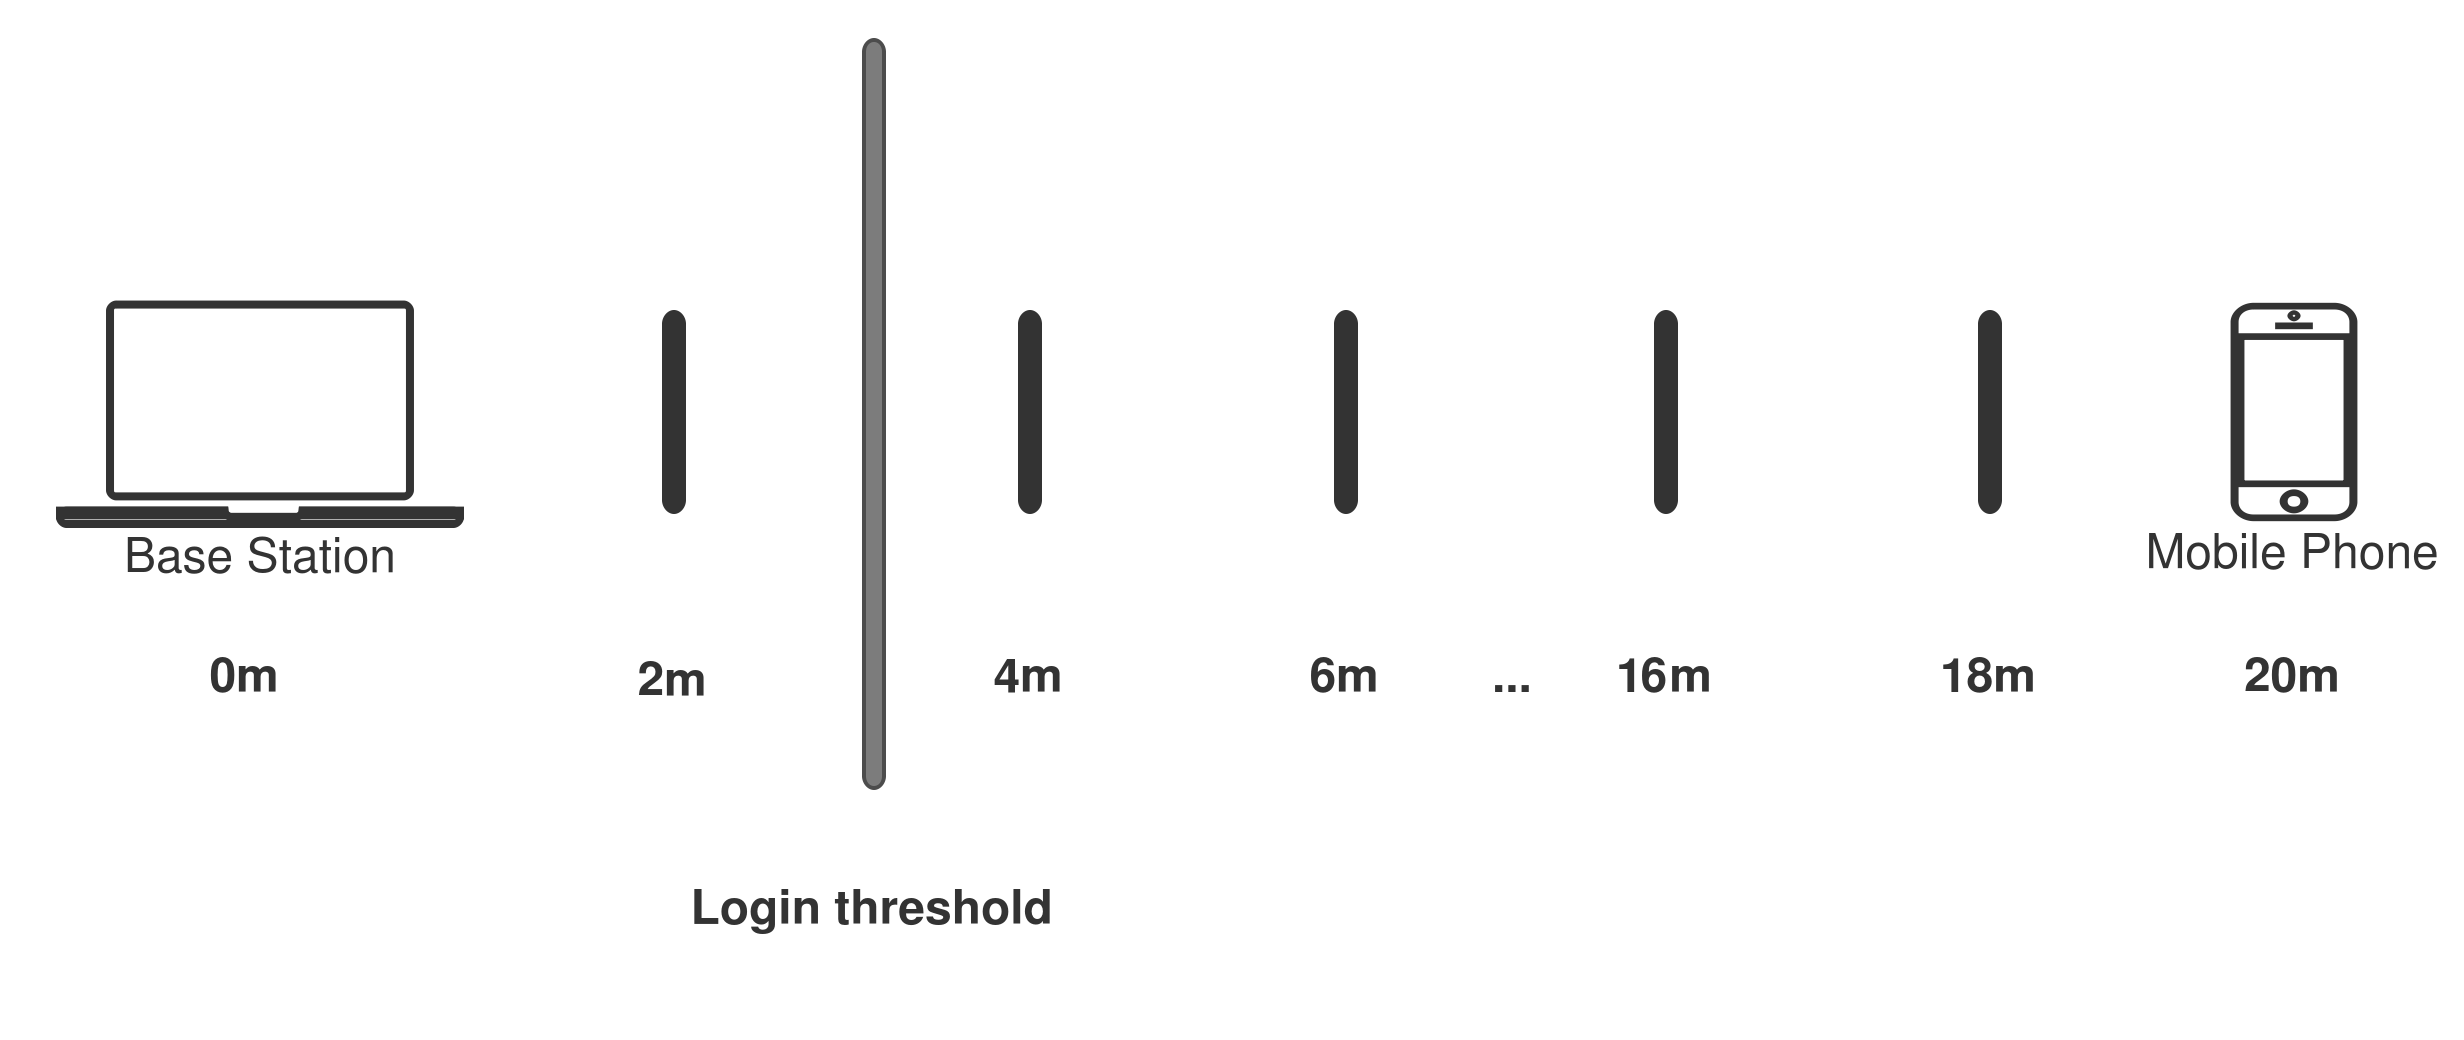
\includegraphics[width=3in]{img/distance}
	\caption{ Distance and threshold }
	\label{fig_distance}
\end{figure}

The base station location is constant. The phone is moved towards the system and RSSI values are measured 60 times at every length, until the device and the base station have the same location. The experiment was conducted 4 times. The phone used is an iPhone 5.

This experiment was conducted in an indoor environment.


\subsubsection{Static distance}
\label{section:MovingTowardsSystem}
As mentioned, RSSI values depends on multiple factors like reflections from environment, antenna, distance and transmission strength. 

The purpose of this scenario is to measure the spread of the RSSI values from a static distance. We collect data for 20 minutes with the phone being approximately 3 meters away from the base station under the entire scenario.

The phone used is a Nexus 5 using Android L and the experiment was conducted in a regular indoor environment and in a noisy indoor environment. The purpose of the change in environment is to see how noise impacts the result.


